\documentclass[12pt]{article}
\usepackage[utf8]{inputenc}
\usepackage[russian]{babel}
\usepackage{amssymb}
\usepackage{systeme}
\usepackage{amsmath}
\usepackage{amsthm}
\usepackage{graphicx}
\usepackage{mathtools}
\usepackage{bbold}
\usepackage{enumitem}
\usepackage{collectbox}
\usepackage{multicol}
\usepackage[margin=0.5in]{geometry}
\usepackage{tabularx}
\usepackage[scr=boondoxo,scrscaled=1.05]{mathalfa}
\usepackage{stackengine}
\usepackage{wrapfig}

\title{Конспекты по линейной алгебре, 2 сем}
\author{Пак Александр}

%----ENVIRONMENTS--------------%
\newtheorem{theorem}{Теорема}[subsection]
\renewcommand{\thetheorem}{\arabic{theorem}}
\newtheorem{lemma}{Лемма}[subsection]
\renewcommand{\thelemma}{\arabic{lemma}}
\newtheorem{defin}{Определение}[subsection]
\renewcommand{\thedefin}{\arabic{defin}}
\newtheorem*{stat}{Утверждение}
\newtheorem{corollary}{Следствие}[theorem]
\renewcommand{\thecorollary}{\arabic{corollary}}
\let\vec\overline

\newenvironment{mylist}{\begin{enumerate}[noitemsep, nolistsep]}{\end{enumerate}}

\theoremstyle{remark}
\newtheorem*{remark}{Замечание}

\theoremstyle{definition}
\newtheorem*{examples}{Примеры}

%-------------------------------%

%------COMMANDS-----------------%
\newcommand{\N}{\numberset{N}}
\newcommand{\Q}{\mathbb Q}
\newcommand{\R}{\mathbb R}
\newcommand{\Z}{\mathbb Z}
\newcommand{\0}{\mathbb{0}}
\newcommand{\mybox}{
	\collectbox{
		\setlength{\fboxsep}{1pt}
		\fbox{\BOXCONTENT}
	}
}
\newcommand{\E}{\mathcal{E}}
\newcommand{\A}{\mathcal{A}}
\newcommand{\B}{\mathcal{B}}
%-------------------------------%

\graphicspath{ {./imgs/} }
\setlength{\parindent}{0ex}
\linespread{1.2}

\begin{document}
	\pagenumbering{gobble}
	\maketitle
	\newpage
	\pagenumbering{arabic}
	\setcounter{section}{6}
	\tableofcontents
	\newpage
	
	\section{Линейные отображения}
	
	\subsection{Основные определения}
	\begin{defin}
		$U, V$ -- линейные пространства над полем $K(\R/ \mathbb{C})$\\
		Линейным отображением $\A$ называется $\A: U \rightarrow V$, обладающее свойством линейности:\\
		$\forall \lambda \in K, \forall u, v \in U\\ 
		\A(u + \lambda v) = \A(u) + \lambda \A(v)$
	\end{defin}
	
	\begin{remark}\hfill
		\begin{mylist}
			\item Записываем не $\A(u)$, а $\A u$
			\item "Поточечно" выполняются все арифметические операции, свойственные функциям
			\item $\A\0_U = \0_V$
		\end{mylist}
	\end{remark}
	\begin{examples}\hfill
		\begin{mylist}
			\item $\0$ -- нулевое отображение $U \rightarrow V$\\
			$\forall u \in U: \0u = \0_v$
			\item $\mathcal{E}$ -- тождественное отображение: $V \rightarrow V$\\
			$\forall v \in V: \mathcal{E}v = v$ 
			\item $U = V = P_n$ -- многочлены степени до $n$
			\\$\A: V \rightarrow V$\\
			$\A p = p'(t)$ -- дифференциальный оператор\\
			$\A(p_1 + \lambda p_2) = (p_1 + \lambda p_2)' = p_1' + \lambda p_2' = \A p_1 + \lambda \A p_2$\\
			Линейное отображение 
			$\A = \frac{d}{dt}$
			\item $U = \R^n \ V = \R^m\\
			\A = (a_{i j})_{m\times n}\\
			\A: x\in U \rightarrow y = \A x \in V\\
			x_1 + \lambda x_2 \in \R^n \rightarrow y = \A(x_1 + \lambda x_2) = \A x_1 + \lambda \A x_2$
			\item $U \cong V$. То есть отображение, на котором строится изоморфизм является линейным.
		\end{mylist}
	\end{examples}
	\begin{defin}$\lambda \in K \ \A: U\rightarrow V$\\
		Произведение линейного отображения на скаляр называется линейное отображение \\
		$\B = \lambda \A \\
		\B: U \rightarrow V \ \forall u \in U \ \B u = \lambda \A u$
	\end{defin}
	\begin{defin}
		Суммой линейных отображений $\A, \B: U \rightarrow V$ называется $\mathcal{C}: U \rightarrow V\\
		\forall u \in U \ \mathcal{C}u = \A u + \B u$
		\mybox{
			$\mathcal{C} = \A + \B$
		}
	\end{defin}
	
	\begin{defin}
		$-\A$ -- отображение противоположное $\A$\\
		$\forall u \in U \ (-\A)u = -1 \cdot \A u$
	\end{defin}
	
	$L(U, V) = Hom_K(U, V) = Hom(U, V) = \mathcal{L}(U, V)$\\
	$L(U, V)$ -- множество всех линейных отображений из $U$ в $V$.\\
	Линейное отображение = гомоморфизм с операциями $\lambda \A$ и $\A + \B$\\
	Выполнены свойства 1--8 линейного пространства (проверить самим). \\Значит \mybox{$L(U, V)$ -- линейное пространство}
	\begin{defin}
		$\A \in L(U, V)\\
		Ker\A = \{u \in U \ | \ \A u = \0_v\}$ -- ядро линейного отображения. 
	\end{defin}
	\begin{defin}
		$Im\A =\{v \in V = \A u \ \forall u \in U\} = \\ \{v \in V \ | \  \exists u \in U \ v = \A u\}$ --
		образ линейного отображения.
	\end{defin}
	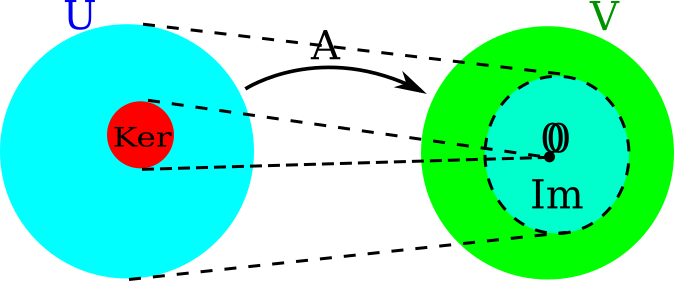
\includegraphics[width=250px]{1}
	
	Упр: $Ker\A$ и $Im\A$ - это подпространства соответственно пространств $U$ и $V$. То есть они замкнуты относительно линейных операций. \\
	Если $Ker\A$ конечномерное подпространство $U$, то \\
	\mybox{$dim \ Ker\A = def\A$} -- дефект линейного отображения.\\
	Если $Im\A$ конечномерное подпространство $V$, то \\
	\mybox{$dimIm\A = rg\A$} -- ранг линейного отображения.
	
	\begin{stat}
		$\A$ изоморфно между $U$ и $V \Leftrightarrow$ 
		\begin{mylist}
			\item $\A \in L(U, V)$
			\item $Im\A = V$
			\item $Ker\A = \{\0\}$ тривиально 
		\end{mylist}
	\end{stat}
	\begin{proof}
		$\A$ изоморфно $\Leftrightarrow$ взаимнооднозначное соответствие + линейность -- $\A\in L(U, V)$\\
		$\0_u \leftrightarrow \0_v$, т. к. изоморфизм $\Rightarrow Ker\A = \{\0\}$\\
		Пусть $Ker\A = \{\0\}$\\
		Докажем инъективность $v_1 = v_2 \Leftrightarrow u_1 = u_2\\
		v_1 = \A u_1 \ v_2 = \A u_2\\
		\0 = v_1-v_2 = \A u_1 - \A u_2 = \A(u_1 - u_2) = \0$ т. к. ядро тривиально.\\
		Сюръективность. $Im\A = V \Leftrightarrow \forall v \in V: \exists u \in U \A u = v$. Последнее и означает сюръекцию.
	\end{proof}
	\begin{defin}
		$\A \in L(U, V)$\\
		--инъективно, если $Ker\A = \{\0 \}$\\
		--сюръективно, если $Im \A = v$\\
		--биективно $\equiv$ изоморфизм, если инъекция + сюръекция.\\
		--эндоморфизм $\equiv$ линейный оператор, если $U \equiv V$\\
		$End_k(V) = End(V) = L(V, V)$\\
		--автоморфизм $\equiv$ эндоморфизм + изоморфизм. \\
		$Aut_k(V) = Aut(V)$
	\end{defin}
	\begin{defin}
		Произведением линейных отображений $\A, \B$ \\
		$\A \in L(W, V) \ \  \B \in L(U, W) \ \
		U \xrightarrow{\B} W \xrightarrow{\A} V$\\
		называется $\mathcal{C} \in L(U, V) : \mathcal{C} = \A\cdot \B$, которое является композицией функций, определяющих отображения $\A$ и $\B$.\\
		$\A\cdot \B = \A \circ \B\\
		\forall u \in U: (\A \B)u = \A(\B u)$\\
		Очевидно, $\mathcal{C}$ -- линейное отображение.
	\end{defin}
	$\Omega \xrightarrow{\mathcal{C}} U \xrightarrow{\B_{1, 2}} W \xrightarrow{\A_{1, 2}} V$\\
	Упр: \begin{mylist}
		\item $\A, \B$ изоморфизмы $\Rightarrow \A\cdot \B$ изоморфизм
		\item $(\A_1 + \A_2)\B = \A_1\B + \A_2\B\\
		\A(\B_1 + \B_2) = \A \B_1 + \A \B_2$ -- дистрибутивность
		\item $\A(\B\mathcal{C}) = (\A \B)\mathcal{C}$ -- ассоциативность
		\item $\lambda \A \B = \A \lambda \B$
	\end{mylist}
	$End(V)$ -- ассоциативная унитарная алгебра\\
	$\mathcal{E}$ -- единица $\mathcal{E}\A = \A\mathcal{E}$
	\begin{defin}
		$\A \in L(U, V)$ изоморфно.\\
		$\forall v \in V \exists! u \in U: v = \A u\\
		\A^{-1}: V \rightarrow U$\\
		\mybox{$\A^{-1}v = u$}\\
		Упр: $\A^{-1}\in L(V, U)$\\
		$\A^{-1} \A = \E_v \ \ \A\A^{-1} = \E_u$
		
	\end{defin}
	$\A\in End(U)$ -- линейный оператор
	
	$\A^{-1}\in End(V)$ -- обратный оператор
	\begin{defin}
		$U_0 \subset U \ \ \A\in L(U, V)$\\
		Сужением линейного отображения $\A$ на линейное подпространство $U_0$ называется \\
		$\A|_{U_0}: U_0 \rightarrow V \ \ \forall u \in U_0 \ \A|_{U_0} u = \A u$
	\end{defin}
	\begin{stat}
		$\A$ изоморфизм $\in L(U, V) \Rightarrow  \A|_{U_0}\in L(U_0, Im(\A|_{U_0}))$ -- изоморфизм
	\end{stat}
	\begin{examples}
		\hfil
		\begin{mylist}
			\item $\0: U\rightarrow U$ -- не сюръекция, не инъекция, эндоморфизм, не автоморфизм.
			\item $\E: U \rightarrow U$ -- автоморфизм
			\item 
			$\A = \frac{d}{dt}$ \  
			$\A: P_n \rightarrow P_n$ -- эндоморфизм, не инъекция, не сюръекция.
			\item $x\in \R^n \rightarrow y = \A x \in \R^n$ -- эндоморфизм. \\
			Сюръекция $\Leftrightarrow rg\A = n \Leftrightarrow \exists \A^{-1} \Leftrightarrow$ инъекция.\\
			То есть автоморфизм.
		\end{mylist}
	\end{examples}
	\begin{theorem}[о $rg$ и $def$ линейного отображения]
		$\A\in L(U, V)$\\
		\mybox{
			$rg\A + def\A = dimU$	
		}
	\end{theorem}
	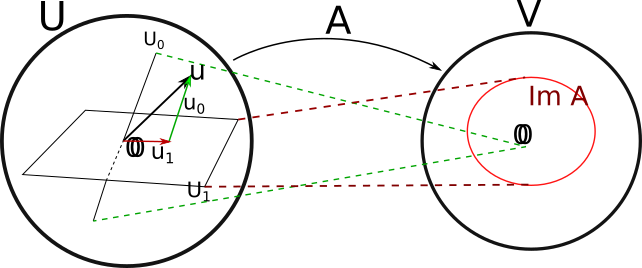
\includegraphics[width=250px]{2}
	\begin{proof}
		$U_0 = Ker\A$\\
		Дополним линейное пространство $U_1$ до пр-ва $U$:\\
		$U = U_0 \oplus U_1 \ \ \ U_1 \cap U_0 = \{ \0 \}\\
		\forall u \in U : u = u_0 + u_1$ (единственным образом)\\
		$\A u = \A u_0 + \A u_1 = \A u_1 \ \ \ \ Im\A = \A(U_1)\\
		\A_1 = \A|_{U_1}: U_1 \rightarrow Im\A$ \\
		$\A_1$ -- изоморфизм? $Im\A_1 = Im\A$ -- сюръекция\\
		$\left.\begin{array}{c}
		\forall w \in Ker\A_1 \in U_1\\
		KerA_1 \subset KerA = U_0
		\end{array}\right \}
		\Rightarrow w \in U_1 \cap U_0 = \{\0\} \Rightarrow Ker\A_1 = \{\0\}\Rightarrow \A_1$ изоморфизм.\\
		$U_1 \cong Im\A \Leftrightarrow dimU_1 = dim(Im\A)$ -- инъекция.\\
		Т. к. $U = U_0 \oplus U_1$, то $dimU = dimU_0 + dimU_1 = \underset{def\A}{dimKer\A} + \underset{rg\A}{dimIm\A}$
	\end{proof}
	\begin{corollary}[Характеристика изоморфизма]
		\ \\
		$\A\in L(U, V)$ Следующие условия эквивалентны:
		\begin{mylist}
			\item $\A$ изоморфно
			\item $dimU = dimV = rg\A$
			\item $dimU = dimV\\
			Ker\A = \{\0\} \Leftrightarrow def\A = 0$
		\end{mylist}
	\end{corollary}
	\begin{corollary}
		$\A \in End(V)$ Следующие условия эквивалентны:
		\begin{mylist}
			\item $\A \in Aut(V)$
			\item $dimV =rg \A$
			\item $Ker\A = \{\0\} \Leftrightarrow def\A = 0$ 
		\end{mylist}
	\end{corollary}
	
	\subsection{Матрица линейного отображения. Изоморфизм алгебр. Преобразование матрицы линейного отображения при замене базиса.}
		$\A \in L(U, V)\\
		\xi_1 \ldots \xi_n$ базис $U$\\
		$\eta_1 \ldots \eta_m$ базис $V$\\
		$\forall u \in U \ u = \sum\limits_{i=1}^{n} u_i\xi_i \leftrightarrow u = \left(
		\begin{array}{c}
		u_1 \\
		\vdots\\
		u_n 
		\end{array} \right)
		\in \R^n(\mathbb{C}^n)$\\
	\begin{tabular}{cc}
		$\A u = \A(\sum\limits_{i = 1}^{n}u_i\xi_i) = \sum\limits_{i=1}^{n}u_i\A\xi_i$ &
		Достаточно знать, как $\A$ работает на базисных векторах $\xi_1\ldots\xi_n$
	\end{tabular}\\ \\
	$Im\A = span(\A\xi_1, \A\xi_2, \ldots, \A\xi_n)$\\
	$$\A\xi_i \in V = \sum_{j=1}^{m}a_{ji}\eta_j \leftrightarrow A_i = \left(
		\begin{array}{c}
			a_{1i}\\
			a_{2i}\\
			\vdots\\
			a_{mi}
		\end{array}\right)
	\in \R^m(\mathbb{C^m})\ \ \ \ 
	a_{ji} \in \R(\mathbb{C})
	$$\\
	\mybox{
		$A = (A_1 \ldots A_i \ldots A_n) = (a_{ij})_{m\times n}$
	}
	матрица линейного отображения $\A$ относительно базисов $(\xi, \eta)$\\\\
	Частный случай: $\A\in End(V): \underset{e_1\ldots e_n}{V} \rightarrow \underset{e_1\ldots e_n}{V}\\
	A = (a_{ji})_{n\times n}$ -- матрица линейного оператора\\
	$A e_i = \sum\limits_{j=1}^{n}a_{ji}e_j$
	\begin{examples}
		\ \\
		\begin{mylist}
			\item
			$\E:\underset{e_1 \ldots e_n}{V} \rightarrow \underset{e_1 \ldots e_n}{V} \ \ \ 
			\E e_i = e_i \leftrightarrow
			\left( 
			\begin{array}{c}
				0\\
				0\\
				\vdots\\
				1\\
				\vdots\\
				0
			\end{array}
			\right)
			\leftrightarrow E_{m\times n} = \left(
				\begin{array}{ccc}
					1 & \ldots & 0\\
					\ldots & 1 & \ldots\\
					0 & \ldots & 1
				\end{array}
			\right)
			$
			\item 
			$$\E: \underset{e'_1\ldots e'_n}{V} \rightarrow \underset{e_1\ldots e_n}{V}$$
			$$
			\E e'_i =  \sum_{j = 1}^{n}t_{ji}e_j \leftrightarrow T_i = 
			\left(
			\begin{array}{c}
			t_{1i}\\
			\vdots\\
			t_{ni}
			\end{array}
			\right)$$
			$$
			[ \E ] _e = T = 
			\left(
			\begin{array}{c}
			t_{1i}\\
			\vdots\\
			t_{ni}
			\end{array}
			\right)
			= T_{e\rightarrow e'}
			$$
			\item \ \\
			\begin{multicols}{2}
				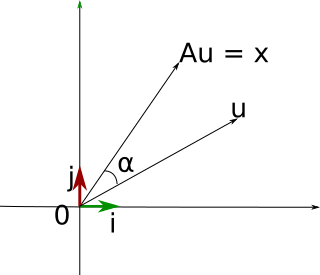
\includegraphics[width=150px]{3}\\
				$\A: \R^2 \rightarrow \R^2\\
				v = \A u$\\
				Поворот векторов в плоскости на угол $\alpha$. \\
				Очевидно, линейный оператор.
			\end{multicols}
			\begin{multicols}{2}
				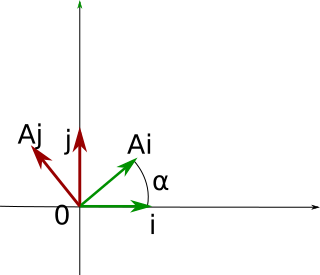
\includegraphics[width=150px]{4}\\
				$
				\A_i = \cos\alpha i + \sin\alpha j \leftrightarrow 
				\left(
				\begin{array}{c}
				\cos\alpha\\
				\sin\alpha
				\end{array}
				\right)\\
				\A_j = -\sin\alpha i \cos\alpha j \leftrightarrow
				\left(
				\begin{array}{c}
				-\sin\alpha\\
				\cos\alpha
				\end{array}
				\right)\\
				\A \leftrightarrow A = 
				\left(
				\begin{array}{cc}
				\cos\alpha & -\sin\alpha\\
				\sin\alpha & \cos\alpha
				\end{array}
				\right)
				$
			\end{multicols}
			\item 
			\begin{multicols}{2}
			$\A: \overset{1, t, t^2}{p_2} \rightarrow  \overset{1, t, t^2}{p_2}\\
			\A = \frac{d}{dt}\\
			\A1 = 1' = 0 \leftrightarrow 
			\begin{pmatrix}
				0\\0\\0
			\end{pmatrix}
			\\
			\A t = t' = 1 \leftrightarrow
			\begin{pmatrix}
				1\\0\\0
			\end{pmatrix}
			\\
			\A t^2 = (t^2)' = 2t \leftrightarrow 
			\begin{pmatrix}
				0\\2\\0
			\end{pmatrix}\\
			\A \underset{(1, t, t^2)}{\leftrightarrow}
			\begin{pmatrix}
				0 & 1 & 0\\
				0 & 0 & 2\\
				0 & 0 & 0
			\end{pmatrix}
			$
			\end{multicols}
			$\A: \underset{1, t, t^2}{p_2} \rightarrow \underset{1, t}{p_1}\\
			\A = \frac{d}{dt} \leftrightarrow A = \begin{pmatrix}
				0 & 1 & 0\\
				0 & 0 & 2
			\end{pmatrix}$
	\end{mylist}
	\end{examples}
	\begin{stat}
		$L(U, V) \cong M_{m\times n}$\\
		(Линейное пространство матриц с вещ.(компл.) элементами размерности $m\times n$. 
	\end{stat}	
	\begin{proof}
		Изоморфизм $\equiv$ биекция + линейность.\\
		Биекция. $\A \rightarrow A_{m\times n}$ -- поняли, как сопоставлять.\\
		Теперь обратно. Пусть $A_{m\times n} = (a_{ij})$\\
		\begin{tabular*}{\textwidth}{c @{\extracolsep{100pt}} c}
			$U \ \xi_1\ldots \xi_n$ базис & $\A: U\rightarrow V$\\
			$V \ \eta_1\ldots \eta_m$ базис &
			$\A\xi_i = \sum\limits_{j=1}^{m}a_{ji}\eta_j \in V$
		\end{tabular*}\\
		$
		\forall u \in U \ u = \sum\limits_{i = 1}^{n}u_i\xi_i
		\\
		\A u = \sum\limits_{i = 1}^{n}u_i\A\xi_i \in V \Rightarrow \A \in L(U, V)
		$
		$\A, \B \leftrightarrow A, B\\
		\forall \lambda \in K \ \A + \lambda\B \overset{?}{\leftrightarrow} A + \lambda B$\\
		$$ (\A + \lambda\B)\xi_i = \A\xi_i + \lambda\B\xi_i = \sum_{j = 1}^{m}a_{ji}n_j + \lambda
		\sum_{j = 1}^{m}b_{ji}\eta_j = \sum_{j=1}^{m}(a_{ji} + \lambda b_{ji})\eta_j \leftrightarrow
		c_i = A_i + \lambda B_i \leftrightarrow A + \lambda B \Rightarrow$$ линейность $\Rightarrow$ изоморфизм.
	\end{proof}
	$\A + \lambda \B \leftrightarrow A + \lambda B\\
	\A\B \leftrightarrow A\cdot B\\
	\A, \A^{-1} \leftrightarrow A, A^{-1}\\
	End(V) \cong M_{n\times n}$ -- ассоциативные унитарные алгебры. (Координатный изоморфизм).\\
	Алгебры изоморфны, т.к. сохраняются свойства дистрибутивности, ассоциативности и т. д.
	\\
	
	\textit{Я не особо понял, что мы дальше делаем, но у меня это записано}\\
	\begin{tabular}{cc}
		$U \xi_1\ldots\xi_n$ & $\forall u \in U \leftrightarrow u = \begin{pmatrix}
		u_1\\
		\vdots\\
		u_n
		\end{pmatrix}$\\
		$V \eta_1\ldots\eta_m$ &
		$u = \sum\limits_{i=1}^{n}u_i\xi_i$
	\end{tabular}
	
	$\forall v\in V \leftrightarrow v = \begin{pmatrix}
		v_1\\
		\vdots\\
		v_m
	\end{pmatrix}\\	
	v = \sum\limits_{j=1}^{m}v_j\eta_j\\
	\A\in L(U, V) \underset{\xi, \eta}{\leftrightarrow} A\\
	\sum\limits_{j=1}^m v_j\eta_j = v = \A u = \sum\limits_{i=1}^n u_i\A\xi_i = \sum\limits_{i=1}^n u_i
	\sum\limits_{j=1}^m a_{ji}\eta_j = \sum\limits_{j=1}^m (\sum\limits_{i=1}^n u_i a_{ji})\eta_j$\\
	Так как координаты определяются единственным образом:\\
	\mybox{ 
		$ v_j = \sum\limits_{i=1}^n a_{ji}u_i $ 
	} 
	$\leftrightarrow$ 
	\mybox{$v = Au$} $\leftrightarrow v = \A u$

	\begin{examples}\ \\
		\begin{mylist}
			\item 
			$\A$ поворот на угол $\alpha$\\
			$(i, j) \leftrightarrow A = \begin{pmatrix}
				\cos\alpha & -\sin\alpha\\\sin\alpha & \cos\alpha
			\end{pmatrix}$
			\\
			\begin{tabular}{lcc}
				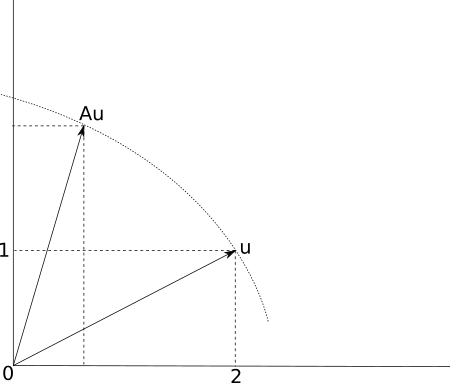
\includegraphics[width=200px]{5} &
				$\alpha=45^{\circ}$ &
				$A = \begin{pmatrix}
				\frac{\sqrt2}{2} & -\frac{\sqrt2}{2}\\
				\frac{\sqrt2}{2} & \frac{\sqrt2}{2}\end{pmatrix}$\\
			$\mathscr{u} \leftrightarrow u = \begin{pmatrix}2\\1\end{pmatrix}$
			\end{tabular}
			\\
			$\mathscr{v} = \A \mathscr{u} \leftrightarrow v = Au = \begin{pmatrix}
				\frac{\sqrt2}{2} & -\frac{\sqrt2}{2}\\
				\frac{\sqrt2}{2} & \frac{\sqrt2}{2}
			\end{pmatrix}\begin{pmatrix}2\\1\end{pmatrix} = \begin{pmatrix}
				\frac{\sqrt 2}{2}\\
				\frac{3\sqrt 2}{2}
			\end{pmatrix}$\\
			\begin{multicols}{2}
				$i \leftrightarrow \begin{pmatrix}
				1\\0
				\end{pmatrix}$\\
				$\A i \leftrightarrow \begin{pmatrix}
					\frac{\sqrt 2}{2}\\
					\frac{\sqrt 2}{2}
				\end{pmatrix}$\\
				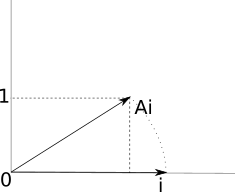
\includegraphics[width=100px]{6}\\
			\end{multicols}
			\item 
			$\A = \frac{d}{dt}: \underset{1, t, t^2}{p_2} \rightarrow \underset{1, t, t^2}{p_2}\\
			A = \begin{pmatrix}
				0 & 1 & 0\\
				0 & 0 & 2\\
				0 & 0&0
			\end{pmatrix}\\
			(\overbrace{3t^3 + 6t + 4}^{u(t)})' = 6t + 6\\
			3t^2 + 6t + 4 = \begin{pmatrix}
				4\\6\\3
			\end{pmatrix}\\
			\A\mathscr{u} \leftrightarrow \begin{pmatrix}
				0&1&0\\0&0&2\\
				0&0&0
			\end{pmatrix}\cdot
			\begin{pmatrix}
				4\\6\\3
			\end{pmatrix}
			= \begin{pmatrix}
				6\\6\\0
			\end{pmatrix} \leftrightarrow 6 + 6t$
		\end{mylist}
	\end{examples}
	\begin{theorem}[Преобразование матрицы линейного отображения при замене базиса]
		$\A \in L(U, V)$\\
		\begin{tabular}{lll}
			$U$ & $\xi = (\xi_1\ldots\xi_n)$ & -- базисы  $\ \ \ \ \A \xrightarrow{(\xi, \eta)} A$\\
			& $\xi' = (\xi'_1\ldots\xi'_n)$
		\end{tabular}\\
		$T_{\eta\rightarrow\eta'}$ -- матрица перехода\\
		\begin{tabular}{lll}
			$V$ & $\eta = (\eta_1\ldots\eta_m)$ & -- базисы  $\ \ \ \ \A \xrightarrow{(\xi', \eta')} A'$\\
			& $\eta' = (\eta'_1\ldots\eta'_m)$
		\end{tabular}\\
		\mybox{
			$\A' = T^{-1}_{\eta\rightarrow\eta'} \cdot A \cdot T_{\xi\rightarrow\xi'}$	
		}
	\end{theorem}
	Ну видимо сейчас доказательство, но я не уверен.
	\begin{proof}\ \\
		\begin{tabular}{c c c}
 			$\underset{\xi_1\ldots\xi_n}{U}$ & \stackanchor{$\xrightarrow{\A}$}{$\rightharpoonup$} & $\underset{\eta_1\ldots\eta_m}{V}$\\
			$\E_u \uparrow \upharpoonright$ & & $\downharpoonleft \uparrow \E_v$\\
			$\underset{\xi'_1\ldots\xi'_n}{U}$ & $\xrightarrow{\A}$ & $\underset{\eta'_1\ldots\eta'_m}{V}$
		\end{tabular}
		\\\\
		$\A = \E^{-1}_v\A\E_u\leftrightarrow A' = T^{-1}_{\eta\rightarrow\eta'}AT_{\xi\rightarrow\xi'}\\
		\A\B \leftrightarrow AB\\
		\A^{-1}\leftrightarrow A^{-1}\\
		\E^{-1}_v \leftrightarrow T^{-1}_{\eta\rightarrow\eta'}$ Смотри пример 2
	\end{proof}
	\begin{corollary}
		\ \\
		$\A\in End(V) \ \ \ \A: \underset{e_1\ldots e_n}{V} \rightarrow \underset{e_1\ldots e_n}{V}\\
		e_1\ldots e_n$ базис $V \leftrightarrow A\\
		e'_1\ldots e'_n$ базис $\leftrightarrow A'\\
		\A: \underset{e'_1\ldots e'_n}{V} \xrightarrow{A'} \underset{e'_1\ldots e'_n}{V}\\
		T = T_{e\rightarrow e'}$\\
		\mybox{$A' = T^{-1}AT$}
	\end{corollary}
	\begin{remark}
		В условиях теоремы $v = \A u \begin{array}{c}
			\xleftrightarrow{(\xi, \eta)} v = Au\\
			\xleftrightarrow{(\xi', \eta')} v' = A'u
		\end{array}\\
		V = T_{\eta\rightarrow\eta'} V'\\
		U = T_{\xi\rightarrow\xi'} U'\\
		T_{\eta\rightarrow\eta'}v' = AT_{\xi\rightarrow\xi'}u'\\
		v' = \underset{A'}{\boxed{T^{-1}_{\eta\rightarrow\eta'}AT_{\xi\rightarrow\xi'}}u'}
		$
	\end{remark}
	\subsection{Инварианты линейного отображения}
	\textbf{Инвариант - свойство, которое сохраняется при некоторых определенных преобразованиях}\\
	$\mathscr{v} = \A\mathscr{u} \leftrightarrow v = Au$\\
	Форма записи действия линейного отображения на вектор инвариантна относительно замены базиса.\\
	$v' = A'u'$
	\begin{defin}
		$A_{m\times n}$\\
		$ImA = span(A_1, A_2,\ldots A_n) = \{\sum\limits_{i = 1}^n \alpha_i A_i|\alpha_i\in K\} = \\
		\{y = Ax \in \R^m(\mathbb{C}^m)| x\in \R^n(\mathbb{C}^n)\}$\\
		$x = \begin{pmatrix}
			\alpha_1\\\vdots\\\alpha_n
		\end{pmatrix}\\
		rgA = dimImA$ --- ранг матрицы\\
		$KerA = \{x\in\R^n(\mathbb{C}^n)|Ax = \0 \} =$ \{множество решений СЛОУ \} --- ядро матрицы\\
		$dimKerA = n-rgA = defA$ --- дефект матрицы\\
		$\boxed{rgA + defA = n}$ --- аналогично теореме о ранге и дефекте
	\end{defin}
	\begin{theorem}
		$\forall \A \in L(U, V)$\\
		\fbox{
			\parbox{73px}{
				$rg\A = rg A$\\
				$def\A = def A$
			}
		}, \\
		где матрица $A$ -- матрица линейного отображения в некоторых базисах пространств $U$ и $V$.\\
		$rg\A$, $def\A$ инвариантны относительно выбора базиса.
	\end{theorem}
	\begin{proof}
		$\A\leftrightarrow\underset{(\xi, \eta)}{A} \xi = (\xi_1\ldots\xi_n)$ базис $U$\\
		$\eta = (\eta_1\ldots\eta_m)$ базис $V$\\
		$Im\A = span(\A\xi_1\ldots\A\xi_n)\\
		\A\xi_i$\stackanchor{$\leftrightarrow$}{$\cong$}$A_i$\\
		Координатный изоморфизм.\\
		Пусть $rgA = k \Rightarrow k$ столбцов линейно независимы, а остальные -- их линейная комбинация.\\
		По свойствам изоморфизма это означает, то из $\A\xi_1\ldots\A\xi_n \ \  k$ линейно независимые, а остальные -- их линейная комбинация $\Rightarrow rg\A = dimIm\A = k\\$
		\belowbaseline[-10pt]{$\begin{matrix}
			dimU\\
			\parallel\\
			n
		\end{matrix}$
		} = \belowbaseline[-10pt]{
			$\begin{matrix}
				rg\A\\
				\parallel\\
				rgA\\
				\parallel\\
				k
			\end{matrix}$
		} $+ def\A\\
		def\A = n-rgA = n-k = dim$ пространства решений $Ax=0 = defA$ 
	\end{proof}
	\begin{corollary}
		$\A$ изоморфизм $\Leftrightarrow A$ невырожденная ($\exists A^{-1}$), где $A$ матрица в некотором базисе.
	\end{corollary}
	\begin{proof}
		Изоморфизм $\Leftrightarrow$ \stackanchor{$defA = 0$}{$dimU = dimV$} $\Leftrightarrow rgA = n \Leftrightarrow A$ невырожденная. 
	\end{proof}
	\begin{theorem}
		$det\A$ не зависит от выбора базиса пространства $V$ (т.е. является инвариантом относительно выбора базиса). И при этом $det\A = detA$, где $A$ -- матрица оператора $\A$ в некотором базисе.
	\end{theorem}
	\begin{proof}
		$V \ e_1\ldots e_n\\
		det\A = det(\A e_1\ldots\A e_n)\\
		\A e_k = \sum\limits_{i_k=1}^n a_{i_k k}e_{i_k} \xrightarrow{A = (a_{ij})} A_k = \begin{pmatrix}
			a_{1k}\\\vdots\\a_{nk}
		\end{pmatrix} = $
		($det$ $n$-форма, т. е. полиномиальная форма) \\
		$ = \sum\limits_{i_1 = 1}^n\sum\limits_{i_2 = 2}^n\ldots\sum\limits_{i_n = n}^n a_{i_1 1}a_{i_2 2}\ldots a_{i_n n}
		\ det(e_{i_1}, e_{i_2}\ldots e_{i_n}) = $ 
		($n$-форма -- 2 одинаковых аргумента $\Rightarrow det = 0$)$\\
		 = \sum\limits_{\sigma = (i_1\ldots i_n)} a_{i_1 1} a_{i_2 2}\ldots a_{i_n n} 
		 \overbracket{det(\underset{\text{все разные}}{e_{i_1}\ldots e_{i_n}})}^{(-1)^{\E(\sigma)} \ \ det(e_1\ldots e_n) = 1}
		 = \sum\limits_{\sigma = (i_1\ldots i_n)}(-1)^{\E(\sigma)} a_{i_1 1} a_{i_2 2}\ldots a_{i_n n} = det A$\\\\
		 $e'_1\ldots e'_n $ базис $V\\
		 T = T_{e\rightarrow e'}\\
		 det\A = det A' \overset{?}{=} det A\\
		 A' = T^{-1} A T\\
		 det A' = det T^{-1} \cdot detA \cdot det T = det A$
	\end{proof}
	\begin{defin}
		$A, B$ называются подобными, если \\
		$\exists $ невырожденная $C: B = C^{-1} A C$
	\end{defin}
	\begin{examples}
		Матрицы линейного оператора в разных базисах подобны\\
		$A' = T^{-1}AT$\\
		$A, B$ подобны $\Rightarrow det A = det B$
	\end{examples}
	\begin{corollary}
		$f$ -- $n$-форма на $V\\
		\forall \xi_1\ldots\xi_n \ \ \forall \A \in End(V)\\
		\Rightarrow \boxed{f(\A\xi_1\ldots\A\xi_n) = det\A \ f(\xi_1\ldots\xi_n)}$
	\end{corollary}
	\begin{proof}
		$f(\A\xi_1\ldots\A\xi_n) = \\
		\underset{n\text{-форма}}{
		g(\xi_1\ldots\xi_n)} = det(\xi_1\ldots\xi_n)\cdot g(e_1\ldots e_n) = \\
		det(\xi_1\ldots\xi_n)\cdot \underset{\text{смотри док-во теоремы}}{f(\A e_1\ldots \A e_n)} = 
		det(\xi_1\ldots\xi_n)\sum\limits_\sigma (-1)^{\E(\sigma)} a_{i_1 1}\ldots a_{i_n n}\cdot f(e_1\ldots e_n) = \\
		\A e_k = \sum\limits_{k = 1}^n a_{i_k k}e_{i_k} =
		\underbracket{det(\xi_1\ldots\xi_n)f(e_1\ldots e_n)}_{f(\xi_1\ldots\xi_n)}\underbracket{det A}_{det\A}
		$
	\end{proof}
	\begin{remark}
		$A$ -- линейный оператор, $B_{n\times n}\\
		AB = (AB_1 \ AB_2 \ldots AB_n)\\
		det(AB) = det(AB_1 \ldots AB_n) = \\
		= detA\cdot det(B_1\ldots B_n) = detA \cdot det B$
	\end{remark}
	\begin{corollary}
		$\A, \B \in End(V)\\
		det(\A\B) = det\A \cdot \B$
	\end{corollary}
	\begin{proof}
		$det(\A\B) = det(AB) = detA\cdot detB = det\A \cdot det\B$
	\end{proof}
	\begin{corollary}
		$\A\in Aut(V)\\
		\Leftrightarrow det\A \neq 0$\\
		Причем $det\det\A^{-1} = \frac{1}{det\A}$
	\end{corollary}
	\begin{proof}
		Из следствия 2\\
		$\A\A^{-1} = \A^{-1}\A = \E\\
		det\A \cdot det\A^{-1} = det\E = 1 \Rightarrow \ldots$
	\end{proof}
	\begin{examples}$V_3$\\
		\begin{multicols}{2}
		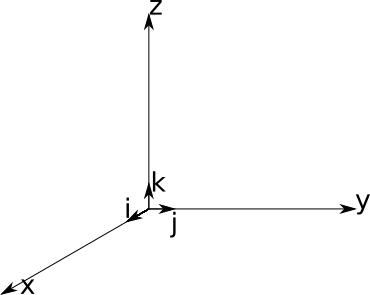
\includegraphics[width=150px]{7}\\	
		$V_{abc \text{--правая тройка}} = \underset{\text{смешанное пр-е}}{\vec{a}\vec{b}\vec{c}} = 
		f(\underset{\text{3-форма}}{\vec{a}\vec{b}\vec{c}})$\\
		$\A\in End(V_3) \ u\in V_3 \rightarrow v = \A u \in V_3$\\
		Как поменяется объем параллелепипеда при линейном преобразовании? 
		\end{multicols}
	$\A (V_{(\vec{a}\vec{b}\vec{c})}) = f(\A\vec{a}, \A\vec{b}, \A\vec{c}) = 
	det\A\cdot f(\vec{a}, \vec{b}, \vec{c}) = det\A \cdot V(\vec{a} \vec{b} \vec{c})\\
	\lambda = |det\A|\ \ \ \ $ Объем увеличится в $\lambda$ раз.\\
	\begin{mylist}
		\item 
		$\A: V_3 \rightarrow V_3$\\
		Оператор подобия\\
		$\forall u\in V_3: \A u = \mu u, \mu \in \R$\\
		\begin{minipage}{0.2\textwidth}
			$A?$
		\end{minipage}
		\begin{minipage}{0.4\textwidth}
			$\A\vec{i} = \mu\vec{i} \leftrightarrow \begin{pmatrix}\mu\\0\\0\end{pmatrix}\\
			\A\vec{j} = \mu\vec{j} \leftrightarrow \begin{pmatrix}0\\\mu\\0\end{pmatrix}\\
			\A\vec{k} = \mu\vec{k} \leftrightarrow \begin{pmatrix}
				0\\0\\\mu
			\end{pmatrix}$
		\end{minipage}
		\begin{minipage}{0.4\textwidth}
			$A = \begin{pmatrix}
				\mu & 0 & 0\\
				0 & \mu & 0\\
				0 & 0 & \mu
			\end{pmatrix}$
		\end{minipage}
	$\lambda = |det\A| = |detA| = |\mu^3|$\newpage
	\item 
	$\A: V_3\rightarrow V_3$\\
	\textbf{Оператор поворота}\\\\
	$\A:  \ \ \ \ \ \begin{matrix}
		\vec{i} \rightarrow e_1 \nearrow \\\vec{j}\rightarrow e_2 \rightarrow\\\vec{k}\rightarrow e_3\searrow
	\end{matrix} \ \ \ 
	\begin{matrix}
		\begin{pmatrix}
			\cos\alpha_1\\
			\cos\beta_1\\
			\cos\gamma_1
		\end{pmatrix}\\
		\begin{pmatrix}
			\cos\alpha_2\\
			\cos\beta_2\\
			\cos\gamma_2
		\end{pmatrix}\\
		\begin{pmatrix}
		\cos\alpha_3\\
		\cos\beta_3\\
		\cos\gamma_3
		\end{pmatrix}\\
	\end{matrix}$\\
	\begin{minipage}{0.5\textwidth}
		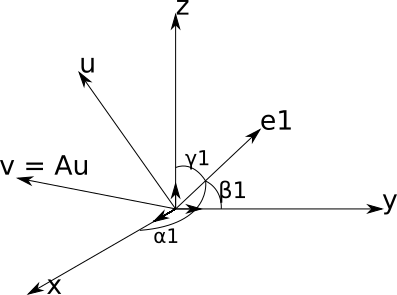
\includegraphics[width=0.5\textwidth]{8}
	\end{minipage}
	\begin{minipage}{0.5\textwidth}
		$|e_i| = 1\\
		(e_i, e_j) = 0\\
		i\neq j$
	\end{minipage}\\\\
	"$\A(V_{\vec{a}\vec{b}\vec{c}})$" $= det\A\cdot V_{\vec{a}\vec{b}\vec{c}} = V_{\vec{a}\vec{b}\vec{c}}\\\\
	A = \begin{pmatrix}
		\cos\alpha_1 & \cos\alpha_2 & \cos\alpha_3\\
		\cos\beta_1 & \cos\beta_2 & \cos\beta_3\\
		\cos\gamma_1 & \cos\gamma_2 & \cos\gamma_3\\
	\end{pmatrix}\\\\
	detA = |\cdots| \underset{\text{Смешанное произведение}}{e_1e_2e_3} = 1$\\
	$(detA)^2 = detA\cdot detA^T = det(AA^T) = det\begin{pmatrix}
		(e_1, e_1) & (e_1, e_2) & (e_1, e_3)\\
		(e_2, e_1) & (e_2, e_2) & (e_2, e_3)\\
		(e_3, e_1) & (e_3, e_2) & (e_3, e_3)\\
	\end{pmatrix}
	= detE = 1\\
	|detA| = 1$
	\end{mylist}
	\end{examples}
	\begin{stat}
		$A, B$ подобные матрицы $\Rightarrow trA = trB$\\
		$trace = $ след
	\end{stat}
	\begin{proof}
		$A, B$ подобные $\Rightarrow\\
		\exists\ C$ невырожденная$: C^{-1}(AC) = B$\\
		$$trB = \sum\limits_{i=1}^n b_{ii} = \sum\limits_{i = 1}^n \sum\limits_{j=1}^n C^{\text{''}-1\text{''}}_{ij}(AC){ji} = 
		\sum\limits_{i = 1}^n \sum\limits_{j=1}^n \sum\limits_{k = 1} ^ n C^{''-1''}_{ij} a_{jk} C_{ki} = 
		\sum_{j=1}^n\sum_{k=1}^n a_{jk} \underbracket{\sum_{i=1}^n C_{ki} C^{''-1''}_{ij}}_{\delta_{kj}} = \sum_{k=1}^n a_{kk} = trA 
		$$
		$\boxed{\delta_{kj} = \left[\begin{matrix}1, k=j\\0, k\neq j \end{matrix} \right.} \ \ CC^{-1} = E$
	\end{proof}
	\begin{defin}
		$tr\A = trA$, где $A$ -- матрица оператора в некотором базисе.\\
		$tr\A = trA = trA'$ --- не зависит от выбора базиса, т.к. $A$ и $A'$ подобны.
	\end{defin}
	\begin{defin}
		$L\subset V \ L$ инвариантно относительно $\A\in End(V)$
		если $\forall u\in L: \A u\in L$
	\end{defin}
	\begin{examples}\ \\
		\begin{mylist}
			\item $\0, V$ инвариантны относительно $\A$
			\item $Ker\A, Im\A $ инвариантны относительно $\A$\\
			\begin{minipage}{0.3\textwidth}
				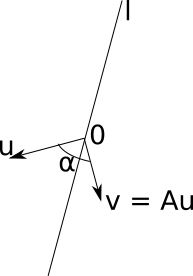
\includegraphics{9}
			\end{minipage}
			\begin{minipage}{0.7\textwidth}
				\begin{flushleft}
					$\A:V_3\rightarrow V_3$\\
					Поворот вектора(пр-ва) относительно оси $l$ на угол $\alpha$
				\end{flushleft}
			\end{minipage}\\
			\begin{minipage}{0.3\textwidth}
				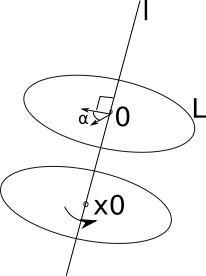
\includegraphics{10}
			\end{minipage}
			\begin{minipage}{0.7\textwidth}
				\begin{flushleft}
					Плоскость $\perp l$ инвариантна относительно $\A$\\
					$P = x_0 + L$ инвариантно
				\end{flushleft}
			\end{minipage}
		\end{mylist}
	\end{examples}
	\begin{theorem}
		$L\subset B \ \ \A\in End(V)$. Линейное пространство инвариантно относительно $\A$\\
		$\Rightarrow \exists$ базис пространства $V$, т.ч. матрица оператора $\A$ в этом базисе\\ будет иметь вид: $A = \left(\begin{array}{c|c}A_1 & A_2\\
		\hline
		\0 & A_3\end{array}\right)\\
		A_1 k\times k$ где $k = dimL$
	\end{theorem}
	\begin{proof}
		$L = span(\underset{\text{базис}}{e_1\ldots e_k})$\\
		Дополним до базиса $V: e_1\ldots e_k e_{k+1}\ldots e_n\\
		e_i \in L \Rightarrow \underset{1\leq i \leq k}{\A e_i}\in L = \sum\limits_{m=1}^k a_{mi}e_m + 
		\sum\limits_{m = k+1}^n 0\cdot e_m
		\leftrightarrow A_i^1 = \begin{pmatrix}
			a_{1i}\\\vdots\\ a_{ki}\\0\\\vdots\\0
		\end{pmatrix}\\
		\underset{k+1\leq i \leq n}{\A e_i} = \sum\limits_{j=1}^n a_{ij} e_j \leftrightarrow 
		A^{2, 3}_i = \begin{pmatrix}
			a_{1i}\\\vdots\\a_{ni}
		\end{pmatrix}
		\Rightarrow A = \begin{pmatrix}
			\boxed{\begin{matrix}
				a_{1i} & \\\vdots & A_i^1 \\a_{ki} & 
				\end{matrix}
			} & \boxed{
				\begin{matrix}
					A^{2, 3}_i\\\ldots
				\end{matrix}
			}\\
			0 & \boxed{\begin{matrix}
			\ldots\\\ldots
			\end{matrix}}
		\end{pmatrix}$
	\end{proof}
	\begin{corollary}
		$V = \bigoplus\limits_{i=1}^m L_i \ \ \ L_i$ инвариантно $\A\\
		\Rightarrow \exists \ $ базис пр-ва $V$, в котором матрица оператора $\A$ будет иметь \underline{блочно-диагональный вид:}\\
		$A = \begin{pmatrix}
			\boxed{A^1} & \ldots & 0\\
			& \boxed{A^2} & \\
			0 & & \boxed{A^n}
		\end{pmatrix}\\
		\left(\underset{\text{размерность матрицы}}{A^i}\right) = dimL_i$
	\end{corollary}
	\begin{proof}
		$L_1 = span(\underset{\text{базис}}{e^1_i\ldots e^{i_k}_i})$\\
		т.к. $\bigoplus$, то базис $V$ -- объединение базисов $L_i\\
		V = span(e^1_1\ldots e^{i_m}_m)\\
		\A^j e_i \in L_i \Rightarrow$ раскладываем по базису $L_i \Rightarrow$\\ на остальных позициях в столбике матрицы оператора будут нули.\\
		$A = \left(
		\begin{array}{c|c|c}
			\overset{\stackrel{L_1}{\underline{1\ldots i_1}}}{\begin{matrix}* & * &*\\ *& * & *\\
				* & * & *\end{matrix}} & 
			\overset{\stackrel{L_2}{\underline{i_1 + 1\ldots i_2}}}
			{\begin{matrix}0 & 0 & 0\\ 0 & 0& 0\\0&0&0\end{matrix}} &
			\begin{matrix}
				0\\0\\0
			\end{matrix} \\
			\hline 
			\begin{matrix}0 & 0 & 0\\ 0 & 0& 0\\0&0&0\end{matrix} 
			& \begin{matrix}* & * &*\\ *& * & *\\
			* & * & *\end{matrix} &
			\left.\begin{matrix}*\\\vdots\\ *\end{matrix}\right\}\\
			\hline
			\begin{matrix}0 & 0 & 0\\ 0 & 0& 0\\0&0&0 \end{matrix}& \begin{matrix}
				0 & 0 & 0\\ 0 & 0& 0\\0&0&0
			\end{matrix} & \begin{matrix}0\\0\\0\end{matrix}
		\end{array}\right) \text{отвечает позиции базисных элементов 
			пр-ва }L_i\text{в базисе }V$
	\end{proof}
	\begin{corollary}
		$V = \bigoplus\limits_{i=1}^m L_i \ \ \ \ L_i$ инвариантно относительно $\A\\
		\A\in End(V)
		\Rightarrow V = \bigoplus\limits_{i=1}^m Im \A|_{L_i}$
	\end{corollary}\newpage
	\begin{proof}
		$V = \bigoplus\limits_{i=1}^m L_i \Rightarrow \forall\ u \in V \ \  \exists! u = \sum\limits_{i = 1}^m u_i \in L_i\\
		Im\A \subset \sum\limits_{i = 1}^m Im\A|_{L_i}\\
		v\in Im\A = \A u = \sum\limits_{i = 1}^m \A u_i \in Im\A|_{L_i}\\
		$
		\textbf{Верно и "$\supset$"}\\
		Пусть $v_i \in Im\A|_{L_i} : v_i = \A u_i, u_i\in L_i\\
		\sum\limits_{i = 1}^m v_i = \sum\limits_{i = 1}^m \A u_i = \A(\sum\limits_{i = 1}^m u_i \in V)\in Im\A\\
		Im\A = \sum\limits_{i = 1}^m Im\A|_{L_i}\\
		\bigoplus$ прямая?\\
		$v_i\in Im\A|_{L_i}\\
		v_i = \A u_i \ \ \ \ u_i \in L_i\\
		\sum\limits_{i = 1}^m v_i = \0 \longleftarrow\\
		\text{Т.к. }L_i $ инвариантна $\Rightarrow \A u_i \in L_i \Rightarrow v_i \in L_i$, но $L_i$ дизъюнктны $\nwarrow \Rightarrow \forall i : v_i = \0\\
		\Rightarrow Im \A|_{L_i}$ дизъюнктны $\Rightarrow \bigoplus$
	\end{proof}
	
\end{document}